\chapter{Application design and implementation}\label{sec:ApplicationDesingAndImplementation}
This chapter describes all important information about created application. First is hardware and software used for developing and testing of the application. Second is structure and description of core parts used in the application. 

\begin{figure}[H]
	\begin{centering}
		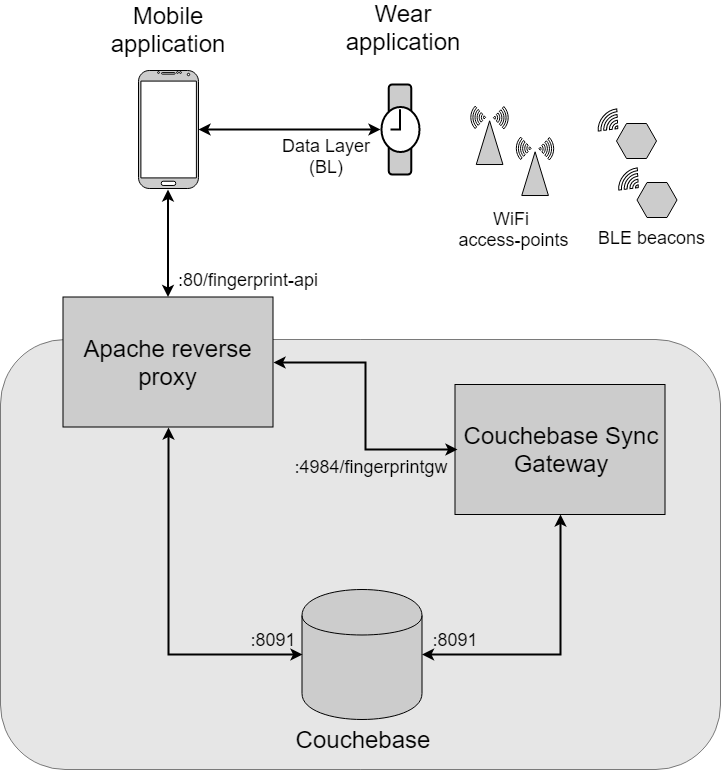
\includegraphics[width=0.6\textwidth]{img/server_architecture}
		\par\end{centering}
	\caption{Application architecture (based on \cite{IILUBLEB})}
	\label{fig01c05}
\end{figure}

\fref{fig01c05} shows basic devices and technologies used in this application. There are three main part of this implementation, mobile, wear and server application. Mobile and wear parts implement scanning for radio signals and are written in Java language for Android system. Server is also programmed in Java to keep implementations close to each other and make future adjustments easier. Main goal of the server is to store scanned data.

\section{Hardware}\label{sec:Hardware}
There are multiple hardware devices used in this application. All of them can be seen on \fref{fig01c05}, where first and the most obvious are smartphone and smartwatch. These devices scan radio signals from WiFi access-points and BLE beacons that are placed in the indoor environment. And a final hardware part is a server holding scanned data from all devices.

\subsection{Smartphone and Smartwatch}\label{subsec:SmartphoneAndSmartWatch}
Both smart devices must support scanning of Bluetooth Low Energy beacons that can be done with Bluetooth 4.0 and higher. Secondary requirements are Wi-Fi, GSM and LTE modules to support more data types than just BLE beacons.

\subsubsection{Phone}\label{subsubsec:Phone}
Main part of the application is developed and tested on Redmi Note 4 from Chinese company Xiaomi. It is running customized version of Android 6.0 called MIUI. Even thought system was customized, in core it is still Android so there are no problems in that regard \cite{XRN4LTE}. This phone has Bluetooth 4.1 with LE support so main requirement for the hardware is met, with all the secondary requirements also met with Wi-Fi 802.11 a/b/g/n, GSM, and LTE support like most modern smartphones would \cite{XRN4FPS}.

One interesting thing about Xioami smartphones is their locked bootloader. It prevents users from any manual updates but most importantly from factory reset. To unlock it owner has to create an account in Xiaomi website and put a request to unlock bootloader. This request is usually processed within two weeks period and there is no actual guarantee of it being approved. After evaluation process is complete user is notified via sms about the result of such request.

\subsubsection{Smartwatch}\label{subsubsec:Smartwatch}
First goal of this thesis was to select smartwatches running on Android Wear 2.0 technology. This iteration is quite new currently, which makes it harder to select proper wear device since there are not so many options. During selection process there were around twenty of watches with this system and only five of them were selected to closer inspection based on few articles \cite{BAWW, BAWW18, BAWW17}.

\begin{table}[h]
	\scriptsize
	\begin{center}
		\begin{tabular}{| m{3cm} | c | c | l |}
			\hline
			Watch & BLE / Wi-Fi & Czech Republic & Problems \\ \hline
			LG W280 Sport & Yes / Yes & No & \begin{tabular}[c]{@{}l@{}} Battery life is one day or less. \\ Too big in size. \end{tabular} \\ \hline
			LG W270 Titanium Style & Yes / Yes & Yes & Battery life is one day or less. \\ \hline
			Huawei Watch 2 & Yes / Yes & Yes & \begin{tabular}[c]{@{}l@{}} First update can take a long time. \\ Slight Bluetooth pairing issues. \end{tabular} \\ \hline
			Polar M600 & Yes / Yes & Yes & \begin{tabular}[c]{@{}l@{}} Polar support complains. \\ Phone synchronization issues. \\ GPS location malfunctions. \end{tabular} \\ \hline
			ASUS ZenWatch 3 & Yes / Yes & No &  \begin{tabular}[c]{@{}l@{}} Strap breaks fast. \\ AW 2.0 update can break the watch. \\ ASUS support complains. \end{tabular} \\ \hline
		\end{tabular}
		\caption{Smartwatch comparison (sources: \cite{LGWSP, LGWST, HW2, PM600, AZW3})}
		\label{tab2}
	\end{center}
\end{table}

Only one smartwatch could be selected out of five displayed in \tref{tab2}. Firstly, wear device had to support BLE and Wi-Fi which all have. Secondly, it must have been sold in Czech Republic (CR) since it makes shipping and warranty easier. Only three of five devices were sold in Czech Republic at that time so others were taken out of the consideration. Final decision was made based on extensive research of customer reviews in shopping sites such as Amazon, CZC, Heureka, Alza, wear official websites \cite{LGWSP, LGWST, HW2, PM600, AZW3} and other tech sites \cite{BAWW, BAWW18, BAWW17}. Finally, selected device was Huawei Watch 2 since there were not too many problems in reviews and other requirements were met.

Initial setup of the wear device was composed of two main parts. First, update wear system which took about one to two hours. Second task was to setup the watch and copy Google account, this is where some problem were discovered. Copying of accounts from Redmi Note 4 to the watch never completed. To fix this problem another smartphone (Huawei Y5 II) was used to copy the account, it was already mentioned that only single device can be connected to smartwatch and connecting to a new one requires factory reset removing all the data. It was needed to pair wear with phone without factory reset which was handled via Android Debug Bridge following this \cite{HtPAWW} article.

Since Google wants to focus also on iOS devices technology Android Wear 2.0 was rebranded to Wear Os by Google to remove confusion in the future \cite{AWITFNM}. This updated was forced on wear devices, updating it to the newest Android version which forced some changes in the development of this solution. First, implementation bug in scanning library was introduced and had to be fixed. Second and bigger problem was inability to deploy new version of the application from Android Studio to the watch. This, for some reason, effects the main computer used to develop this application and it was fixed by using another computer.

\subsection{Radio signal devices}\label{subsec:RSD}
As hardware devices are used BLE beacons, WiFi access-points and Cellular towers. Only first two types of these devices can be placed inside a building and are most commonly used in indoor localization. Signal from cellular towers is only a complimentary data that does not have to be used and cannot be influenced since they are placed by telecommunication companies.

\subsubsection{BLE beacons}\label{subsec:BLEBeacons}
Beacons are small devices that can be easily placed in almost any environment. Only thing they do is send an information packets using Bluetooth and nothing else. They are commonly used in museums, airports and as of late in indoor localization \cite{10TABB}. Beacons have their own battery powering them which can last around a year or two without charging because of the new Bluetooth Low Energy (BLE) standard. This technology drastically reduces power consumption and introduces new configuration
options regarding the advertising interval and the transmitter output power \cite{IPSBOBLE}. More in depth description of this technology and devices was written by Pavel Kriz et al. \cite{IILUBLEB}.

There are multiple beacon manufacturers with their own quality, signal strength, battery life and other hardware differences. Changes can also be found in software (packet) specifications for beacons, meaning data they send have different format but it does not mean other systems cannot see them. Usually some software changes have to be made to detect such beacons but they are documented and not hard to make. Beacons are also usually platform independent, making them work with multiple platforms such as Android or iOS \cite{IPSBOBLE, 10TABB}. Beacons used in this thesis are from a company called Estimote and they are most commonly used.

\begin{figure}[H]
	\begin{centering}
		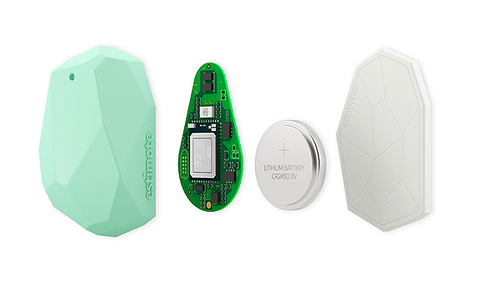
\includegraphics[width=0.6\textwidth]{img/estimote_beacon}
		\par\end{centering}
	\caption{Parts of Estimote beacon (source: \cite{RMPFEB})\label{fig:PartsOfEstimoteBeacon}}
	\label{fig02c05}
\end{figure}

Another important thing to note, Beacons are not connected to the Internet and do not collect any data from devices around them. Meaning all the data have to be processed in another device, most commonly a smartphone, and it also makes Beacon safe to use because there is no need to worry about sensitive data theft \cite{10TABB}.

\subsubsection{WiFi access-points}\label{subsec:WiFi access-points}
WiFi signals are commonly used in indoor localization due to their presence almost anywhere. In this case several WiFi transmitters of the \verb|eduroam| network made by Cisco were used. They are permanently deployed on every floor of a test building and cannot be influenced or changed.

\section{Server}\label{sec:Server}
Implemented application do not necessarily need a server for its core functionality but it is common and faster to run an analysis of the data and other heavy computational work on a different, faster device. Functionality of the server is to serve as a backup of the data and also as a synchronization point to enable other devices to download fingerprints and upload new ones.

The server infrastructure was built in previous years \cite{IILUBLEB} but it was improved for this solution. It uses NoSQL database to save fingerprints. This type of database does not have fixed scheme, making it easy to save all kinds of data. There are many NoSQL databases, around 250 at this time, to choose from. Selected database is called Couchbase, it saves data in JSON files with its own query language similar to SQL. Part of this database can also replicate data between other devices which could be used in the application part. In the end it was deemed too slow and data heavy for usage in the application, creating the need for creation of a middleman API between Android application and Couchbase database.

As \fref{fig01c05} shows server has three main parts to work with. First, already mentioned is Couchbase database to keep scanned data. Second, sync gateway that can synchronize data between devices, not used in this implementation. Both of these part were already implemented in previous years \cite{IILUBLEB}. Final part is web application working as a REST API to send data between the server and mobile application. 

This API is written in Java based framework called Spring to keep the code similar to Android. It was documented using Swagger and it handles two main HTTP routes: \verb|fingerprints| and  \verb|fingerprints-meta|. Before any tasks are issued, mobile application checks data on the server using \verb|fingerprints-meta| route which returns count of new fingerprints and last time specific device saved fingerprints on the server. With this information the application knows how many fingerprints to upload and download, in this specific order, to ensure data is stored first. To prevent device memory exhaustion and connection timeout both of these tasks have specific limits, download can process 100 of fingerprints while upload only 20. Server can also generate data files for analysis, split by technology, time, origin device and other filters. To simplify this generation it is similar loading all fingerprints, meaning it does not create file but prints the data directly into the connection stream.

One last thing to note in \fref{fig01c05} is the connection with sync gateway. Even though it is not used in this implementation for synchronization it is used to save fingerprints into the database. When data is saved into Couchbase directly sync gateway will not display them, that is why the upload must go through the gateway. This is to ensure all previous and next solution can use this feature without loosing any important data.

\section{Application Software}\label{sec:ApplicationSoftware}
Software part for smartphone and smartwatch uses Android system which was already described in \hyperref[sec:WearOS]{Chapter 3}. This section will provide basic information about libraries, technologies and systems used in such applications.

\subsection{AltBeacon Library}\label{subsec:AltBeaconLibrary}
Since Android core does not allow scanning for BLE beacons this feature must be implemented in a library extending system features. There are multiple solutions that can be used to scan for beacons such as Estimote SDK \cite{ESDKfA} which was already used in previous thesis \cite{PMRIL}. To change things up BLE beacons are found via AltBeacon Library \cite{ABL}.

Since there was no open and inter-operable specification for proximity beacons, Radius Networks has created the AltBeacon specification as a proposal to solve this issue. It is an open and free specification for BLE beacons with focus to create an open, competitive market for implementation of these devices \cite{AltB}. Basic configuration of this library can scan for beacons based on this standard and it also supports Eddystone beacons which is Google's open source format. To support already mentioned Estimote beacons this library configuration must be altered to support their detection. Luckily this function can be easily modified to support different kinds of beacons by just one following line of code \cite{ABL, EDDF}.

\begin{lstlisting}[caption=Code to enable all beacon types]
beaconManager.getBeaconParsers().add(
	new BeaconParser().setBeaconLayout("m:2-3=0215,i:4-19,
		i:20-21,i:22-23,p:24-24"));
\end{lstlisting}

This library uses publish-subscribe design pattern, meaning one scan data is send to multiple clients if they listen for them. Using this approach has an advantage of eliminating the need to run a scan per client. Update to Android 8 introduced a bug in this feature making it unable to confirm the registration of client so the scanner has to be reworked thus postponing the data collection and analysis.

\subsection{Database}\label{subsec:Database}
This solution makes use of two different types of databases to store all the Fingerprint data for calculations. First, is SQLite database implemented in Android mobile application to save Fingerprints from smartphone and smartwatch. This database is default implementation and most commonly used in Android applications. Second database type is Couchbase implemented on the server \verb|beacons.uhk.cz| to keep all Fingerprint data in one place and this enable synchronization and data analysis.

\subsubsection{SQLite database}\label{subsec:SQLiteDatabase}
SQL (Structured Query Language) is a standard language for storing, manipulating and retrieving data in databases. It is a type of Relational Database, meaning all data is saved into tables with specified rows and columns \cite{WISQLITE}. These tables usually have set amount of rows with specific names that protect from adding wrong data, for example you cannot add data \verb|Person(name, surname, eye color)| into table \verb|Person(name, surname)| because there is no column named \verb|eye color| in the table.

Structured data is one of the advantages of this database type and it makes calculation faster but usually uses more storage space. Other advantage is that data can be only saved once since they can be connected to each other. It supports complex queries for creating, reading, updating and removing data (CRUD) and better security with user and table management. Some disadvantages of this system can be with complexity and inflexibility of database scheme because it is hard to setup and does not allow other data then is defined in the tables \cite{ERDMS}. Altering schemes in the future can be really complex since there is the need to parse all previous data to the new tables which does not need to have the same scheme as previous ones.

Since SQL with all its features can consume a lot of hardware resources for a smartphone, Android decided to implement lite version of this database. SQLite has the following noticeable features: self-contained, serverless, zero-configuration, transactional \cite{WISQLITE}.

\begin{itemize}
	\item Serverless = does not need second process for the server.
	\item Self-Contained = requires minimal support from operating system.
	\item Zero-configuration = no need for installation or any configuration.
	\item Transactional = data are protected against failed changes (application crashes, power failure, ...).
\end{itemize}

\subsubsection{Couchbase database}\label{subsec:CouchbaseDatabase}
Since SQL based databases can be complex to implement, scale and usually require more data storage space there was a motivation to create so called NoSQL databases. Their most important and significant feature is not having a fixed scheme, that makes them easy to scale and replicate between multiple devices. There are around 225 NoSQL databases at this time and selected Couchbase is one of them \cite{NOSQLDB}.

Couchbase is distributed, document-based database with its own querying language called N1QL. It is a database focused on simple server configuration and easy usage for clients, with built in caching layer and distribution system it does not require any changes in the application. There can be either one server instance of Couchbase or multiple connected to create a database cluster which holds all the data in multiple locations (nodes) \cite{GSWCBS}. This data is saved in JSON file format and usually in readable form without any encryption.

\begin{lstlisting}[caption=JSON format example]
[
	{ "id":"1", "name":"Joe", "lastName":"Doe", "address":{} },
	{ "id":"2", "name":"James", "lastName":"Named", "address":{} }
]
\end{lstlisting}

Since SQL is used for decades and it became standard for working with data in databases, Couchbase embraces this approach and extends it for JSON files, this language is called N1QL. It has all the main features of the SQL with some minor improvements \cite{WINQL}. Currently this language can be used only on the server implementation, meaning Android cannot use this feature. Version for mobile application is called Lite and instead of N1QL so called \verb|views| are used, they are objects containing all the selected data from the documents. Major problem of \verb|views| is being very data heavy which is shown in \hyperref[subsubsec:Comparison]{Comparison} section. That is one of two main points why mobile and wear applications use an SQLite instead of Couchbase. Second point is to differentiate between previous solutions and test data consumption and load speed of SQL database.

\subsubsection{Comparison}\label{subsubsec:Comparison}
Both of these database solutions were tested on Android mobile application to figure out which one is faster and takes less data storage space. As a test 315 fingerprint documents will be loaded and displayed, all of them have more than 500 sub-documents which makes about 150 000 documents. As \tref{tab3} shows SQLite takes less space and is almost three times faster in loading all the documents, that is why it was selected for this project. If Couchbase Lite would have faster query time or supported the use of N1QL it would be preferable solution but it is not at this time.

\begin{table}[h]
	\begin{center}
		\begin{tabular}{| l | c | c |}
			\hline
			Database type & Data size & Loading speed (315 documents) \\ \hline
			SQLite & 15MB & 23 second \\ \hline
			Couchbase without views & 31MB & 65 seconds \\ \hline
			Couchbase with views & 91MB & 65 seconds \\ \hline
		\end{tabular}
		\caption{Couchbase vs SQLite (sources: \cite{LGWSP, LGWST, HW2, PM600, AZW3})}
		\label{tab3}
	\end{center}
\end{table}

Selecting SQL comes with a disadvantage since it does not provide any data synchronization, due to that there must be custom solution created which was already described in \hyperref[sec:Server]{Server} section.

\subsection{TileView}\label{subsec:TileView}
There are multiple ways to display image map in Android, default solutions usually load the whole picture at once. This works for smaller pictures but it does not have to work for bigger ones because the device can run out of memory. To solve this problem it is usually better to try custom library or widget created specifically for displaying such images. One approach is to use 2D or 3D library to display image, these libraries usually work with the image as a whole and implement complex functionality to display it without memory exhaustion. The other approach, also used by Google Maps, is to cut the big image to smaller parts (\verb|tiles|) and display them next to each other. This approach has multiple advantages.

\begin{itemize}
	\item Solves performance issues and enables cartographers to aesthetically pleasing maps without worrying about performance impact.
	\item When user is panning relevant pictures stay displayed while others are loaded, improving user experience.
	\item Every zoom level has its own collection of images, this makes it easy to keep a good quality for all zoom levels.
	\item When zoomed pictures out of the screen do not have to be kept in memory, this cannot be one with single picture.
	\item Zoomed images can have more details.
\end{itemize}

Tiles are usually images that have 265x265 pixels but that is not the requirement. There is one tile with the image displayed for the lowest zoom, level 0, where each zoom increase splits this image into 4 tiles. For practical purposes max zoom level is usually around 21 with almost 4,5 trillion tiles.

\begin{figure}[H]
	\begin{centering}
		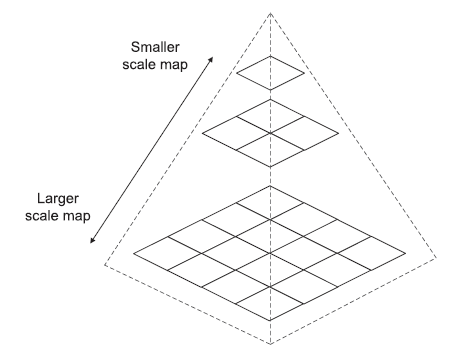
\includegraphics[width=0.6\textwidth]{img/tile_pyramid}
		\par\end{centering}
	\caption{Tile pyramid for zoom levels (source: \cite{WTM})\label{fig:TilePyramid}}
	\label{fig03c05}
\end{figure}

Creating tiles by hand can be really time consuming job even for low zoom levels it can be done automatically by script or program. For example it is possible to create them by slice tool in PhotoShop but this solution support only low level of zoom since it has a limit for amount of such created images. Author of this library provides a solution to this problem using a free tool called ImageMagick, which can resize, crop, cut and create images using a command line making it easy to create a script for all zoom levels required \cite{TileView}.

\begin{lstlisting}[caption=Creating tiles using ImageMagick]
C:\*path to imagemagick*\convert C:\*path to big image*.png 
	-crop 256x256 
	-set filename:tile "%%[fx:page.x/256]_%%[fx:page.y/256]" +repage +adjoin 
	"C:\*path to tile folder*\tile-%%[filename:tile].png"
\end{lstlisting}

This code will split image.png into 256x256 tiles, and name them \enquote{tile-i-j.png}, where \enquote{i} is the column index and \enquote{j} is the row index. More information can be found in the TileView wiki \cite{TileViewWiki}.

\section{Application implementation}\label{sec:ApplicationImplementation}
Implementation of this application is split into two parts, mobile and wear. Both of them have to implement two tasks in order to be able to create fingerprint maps. First, scanner for radio signals which will record Bluetooth Low Energy beacons, WiFi access-points and Cellular towers. Second, communication between both implementation, mobile and wear, to allow sending fingerprint information between them. Those are two core functions for both applications but since the synchronization server is used, mobile part also has to communicate with the server.

Both of these applications are programmed in Java language using Android Studio, each of them has a separate configuration and is aimed to different system versions.

\subsection{Scanner}\label{subsec:Scanner}
Scans for radio signal and creates a fingerprint with specific position, device and selected sensor information. This additional data, especially about the device, will help with analysis by splitting data into groups.

There are multiple parts to this task and most of them are very computational heavy so it is better to implement it in a separate \verb|Thread| to prevent application from freezing. Android provides multiple solutions for running tasks in separate Threads.

\begin{itemize}
	\item AsyncTask - Simple solution mainly focused on short running tasks. This implementation is easily created since it handles basic functions like running task, run code before and after task, publish progress to the main Thread and many more.
	\item Service - Mainly focused on long running tasks and it is run immediately after it is started.
	\item Custom Thread - One of the hardest solutions because developer has to handle all the task related to Threads life-cycle and be careful to prevent creation of multiple unwanted Threads.
	\item JobScheduler - One of the newest implementations, it is focused to schedule task and run them when the device has required resources ready and not immediately.
\end{itemize}

Scanner is run using JobScheduler, it is a new technology and Android wants to develop this feature. Handling scanned data is implemented using publish-subscribe design pattern handled by \verb|BroadcastReceiver|. There are three separate Receivers for each type of signal collected and one more for collecting data from sensors. 

\subsubsection{JobScheduler}\label{subsubsec:JobScheduler}
This feature was introduced in Android 5.0 and it remains under active development with major changes in Android version 7.0. This platform collects information about jobs that need to run across all the applications. Some information collected about specific jobs are: required network access, is the job periodic, should the job be scheduled after device restart and more. This information is used to schedule jobs to run at, or around, the time they were scheduled. JobScheduler is intelligent about running jobs and it uses so called batching, which is combining multiple jobs to reduce battery consumption \cite{AD, SOTAJS}.

\begin{lstlisting}[caption=Schedule Firngerprint scanner job.]
// Building job to run
JobInfo.Builder jobBuilder = new JobInfo.Builder(FingerprintScanner.JOB_ID, new ComponentName(getPackageName(), FingerprintScanner.class.getName()));
jobBuilder.setOverrideDeadline(1000);
jobBuilder.setPersisted(false);
jobBuilder.setExtras(bundle);
// Run created job
JobScheduler jobScheduler = (JobScheduler) getSystemService( Context.JOB_SCHEDULER_SERVICE );
jobScheduler.schedule(jobBuilder.build());
\end{lstlisting}

This code is used to schedule Fingerprint scanner. Firstly, a job has to be created with specific ID and class to contain job code. Secondly, job information are provided: this task should start around a second after scheduling, it is not run after device restart and there are custom data send to it via \verb|setExtras()| function. Finally, job scheduler is loaded and this job is run. One thing to remember is to not create a new instance of JobScheduler class since it is a system service.

\subsubsection{BroadcastReceiver}\label{subsubsec:BroadcastReceiver}
Broadcast messages are send from Android system and other Android applications, similar to the publish-subscribe design pattern. This messages are send when an event occurs such as system boot up, start of device charging or network connectivity change. In addition to system events, custom ones can be created in the application to inform other applications. When a broadcast is sent, the system automatically routes it to application that have subscribed to receive that particular type of broadcast \cite{AD}. Following code illustrates how easy is to send a custom broadcast identified by specific action, which can be system or custom. BLE beacon data is added to be received and parse into Fingerprint. Last line sends the actual broadcast to be received by other applications.

\begin{lstlisting}[caption=Send broadcast with BLE beacons found.]
Intent intent = new Intent();
intent.setAction(ACTION_BEACONS_FOUND);
intent.putParcelableArrayListExtra(ACTION_BEACONS_DATA, foundBeacons);
sendBroadcast(intent);
\end{lstlisting}

Receiving broadcasts in application has two steps. First, register the receiver implementation and specific broadcast message it should receive, this can be done via manifest or dynamically in code. If receiver is registered using manifest, application is launched (if it is not running already) when the broadcast is sent. Second, create an implementation of BroadcastReceiver class that will handle information and data using \verb|onReceive()| function.

There are two BroadcastReceiver used in the Scanner. First, used for WiFi scanning since it is a default Android solution. Second, BLE scanner was modified to use this approach because there are multiple parts of this application that can receive information about found beacons. Other two scanners use Listeners which are interfaces handling communication between system and application.

\subsection{Device communication}\label{subsec:DeviceCommunication}
In this application device communication is used to send fingerprint data between devices using Bluetooth. Mobile application sends information about the fingerprints such as location and scan duration, these values are same for both devices. Wear application will in return send result data after scan was finished to save it into the mobile database.

First implementation of this feature was build upon Bluetooth chat example application from Google. This implementation was using three separate Thread to make connection, authorize it and then to send the data when device was connected. Both devices had to accept the connection to send the data, which is normal, but there were some connection loss issues where one devices was considered connected and sending data while the second device was disconnected and not receiving data. That is why this solution was removed at early development stages and substituted by Google's Data Layer API.

To limit data consumption of this application on wear it does not run constantly. Before any scan is started mobile informs wear to start the application, after this is done mobile sends fingerprint data to wear part of the application which is returned after the scan is done with acquired data.

% Example of this as a picture.

\subsubsection{Data Layer API}\label{subsec:DataLayerAPI}
Data Layer is commonly used by Google to send data between their applications. There is an implementation using this feature called Google Tag manager which is sends data from websites to other Google tools like Analytics or Adwords. In this case is a JavaScript object or variable creating virtual \verb|layer| of website application which contains various \verb|data| points, making its name, \verb|Data Layer| \cite{GTMDL}.

Since it proved as a useful solution it was also implemented for Android and it is a part of Google Play services. The Data Layer API allows to store and retrieve data from different kinds of devices, it this case between mobile phone and wear. There are multiple ways to send data depending on what should be sent \cite{AD}.

\begin{itemize}
	\item Data Item - It provides a data storage that is synchronized between mobile and wearable device. Whenever data changes all devices using this item are then informed about the change and it is identifies by Uri containing creator and path.
	\item Asset - Used to send binary blobs of data, such as images. It takes care of the data transfer automatically using caching to avoid sending the same data multiple times.
	\item Message - Good for sending small amounts of data or remote procedure calls, such as controlling mobile media player from wearable. If the device receiving data is connected sender receives a result code confirming successful data send. Although if the device is disconnected right after receiving the result code this information might not be 100\% precise.
	\item Channel - Transfers large data entities, such as music and movie files. It saves the disk space over Data Item or Asset because it does not create copy of the message on local device before synchronization. It can be also used to transfer streamed data, such as music pulled from a network.
\end{itemize}

This application uses message system and data items, where messages are send to start wear application and confirm its startup and later Fingerprint data are send via data items. Since application may be either in foreground or background there need to be two solutions to receive the data. First, a service that runs when the application is not started or in the background. Second, any activity can implement an interface that will get received data in foreground.

One important thing to note is, to send the data successfully between the devices they must have the same APK signatures, meaning they must be signed by the same key. For example, debug versions of two applications developed on two different computers will not be able to send data due to this restriction.

\subsection{Server communication}\label{subsec:ServerCommunication}
Main task of communicating with the server is to synchronize data on the mobile, downloading previous fingerprints and upload newly scanned ones. This feature uses server api to transfer data and since this is a very data and computational heavy task it is run in a separate thread same as a scanner, also using a JobScheduler. It was already mentioned that server api is documented in Swagger, this tool can also generate android code to communicate with the server based on defined functions in the documentation. This will generate working code without the requirement of using secondary library but the code is unnecessary complex and so this application uses simple library called Retrofit.

Even though the new version of Android Wear OS makes this feature easier to implement on the wear device, it is still used only in the mobile application for one simple reason: to lower power consumption. 

\subsubsection{Retrofit}\label{subsec:Retrofit}
Retrofit is a library turning HTTP API into a Java interface making the implementation simple. Such interface contains calls with parameters based on the api documentation, that can return either raw response or automatically convert the data into Java classes based on configuration. Creating the interface is only one of two parts to make this library working. Second is create an instance of this library's main class with a configuration specific to the api.

\begin{lstlisting}[caption=Retrofit interface example.]
public interface ApiConnection {
	@GET("fingerprints")
	Call<List<Fingerprint>> getFingerprints(@Header("deviceId") String deviceId,
		@Query("timestamp") long timestamp,
		@Query("limit") int limit,
		@Query("offset") long offset);
}
\end{lstlisting}

Small example of Retrofit interface class with a function for getting fingerprints. Firstly, Retrofit must be informed which HTTP call it should use, such as GET, POST, PUT or DELETE, part of this information can also be URL path added to the call, \verb|fingerprints| in this case. Secondly, all of the parameters must inform 
where they should be posted, in header, body or query.

\begin{lstlisting}[caption=Retrofit configuration example.]
Retrofit retrofit = new Retrofit.Builder()
	.baseUrl("http://beacon.uhk.cz/fingerprint-api/")
	.addConverterFactory(JacksonConverterFactory.create())
	.callbackExecutor(Executors.newSingleThreadExecutor())
	.build();
\end{lstlisting}

There is only one required configuration to make retrofit work and that is defining base URL so the library knows where to post the calls. Some other configurations might be adding data converter which converts the data from Json to Java classes, run calls in different threads or create custom HTTP client.

\subsection{Application screens}\label{subsec:ApplicationScreens}
Mobile application has three screens, map and scanner, surrounding devices, synchronization screen and wear application has only one containing information about the scan.

\subsubsection{Map and scanner}\label{subsec:MapAndScanner}
This screen is the core of this application it shows the map of building floor with fingerprint positions as markers. Map is implemented using TileView library described previously in this chapter. It is used to display locations of fingerprint measurements and enable to create new ones or delete previous ones. Deleting was not supposed to be part of the implementation but it proved useful when one or both of the devices collected \enquote{broken} fingerprints, which are usually created by failure in WiFi scanning or failing o send data from mobile to wear device. Deleting removes last created fingerprint group, meaning it deletes one per device type, this is possible because fingerprints have their specific scan id connecting them together.

\begin{figure}[h!]
	\begin{centering}
		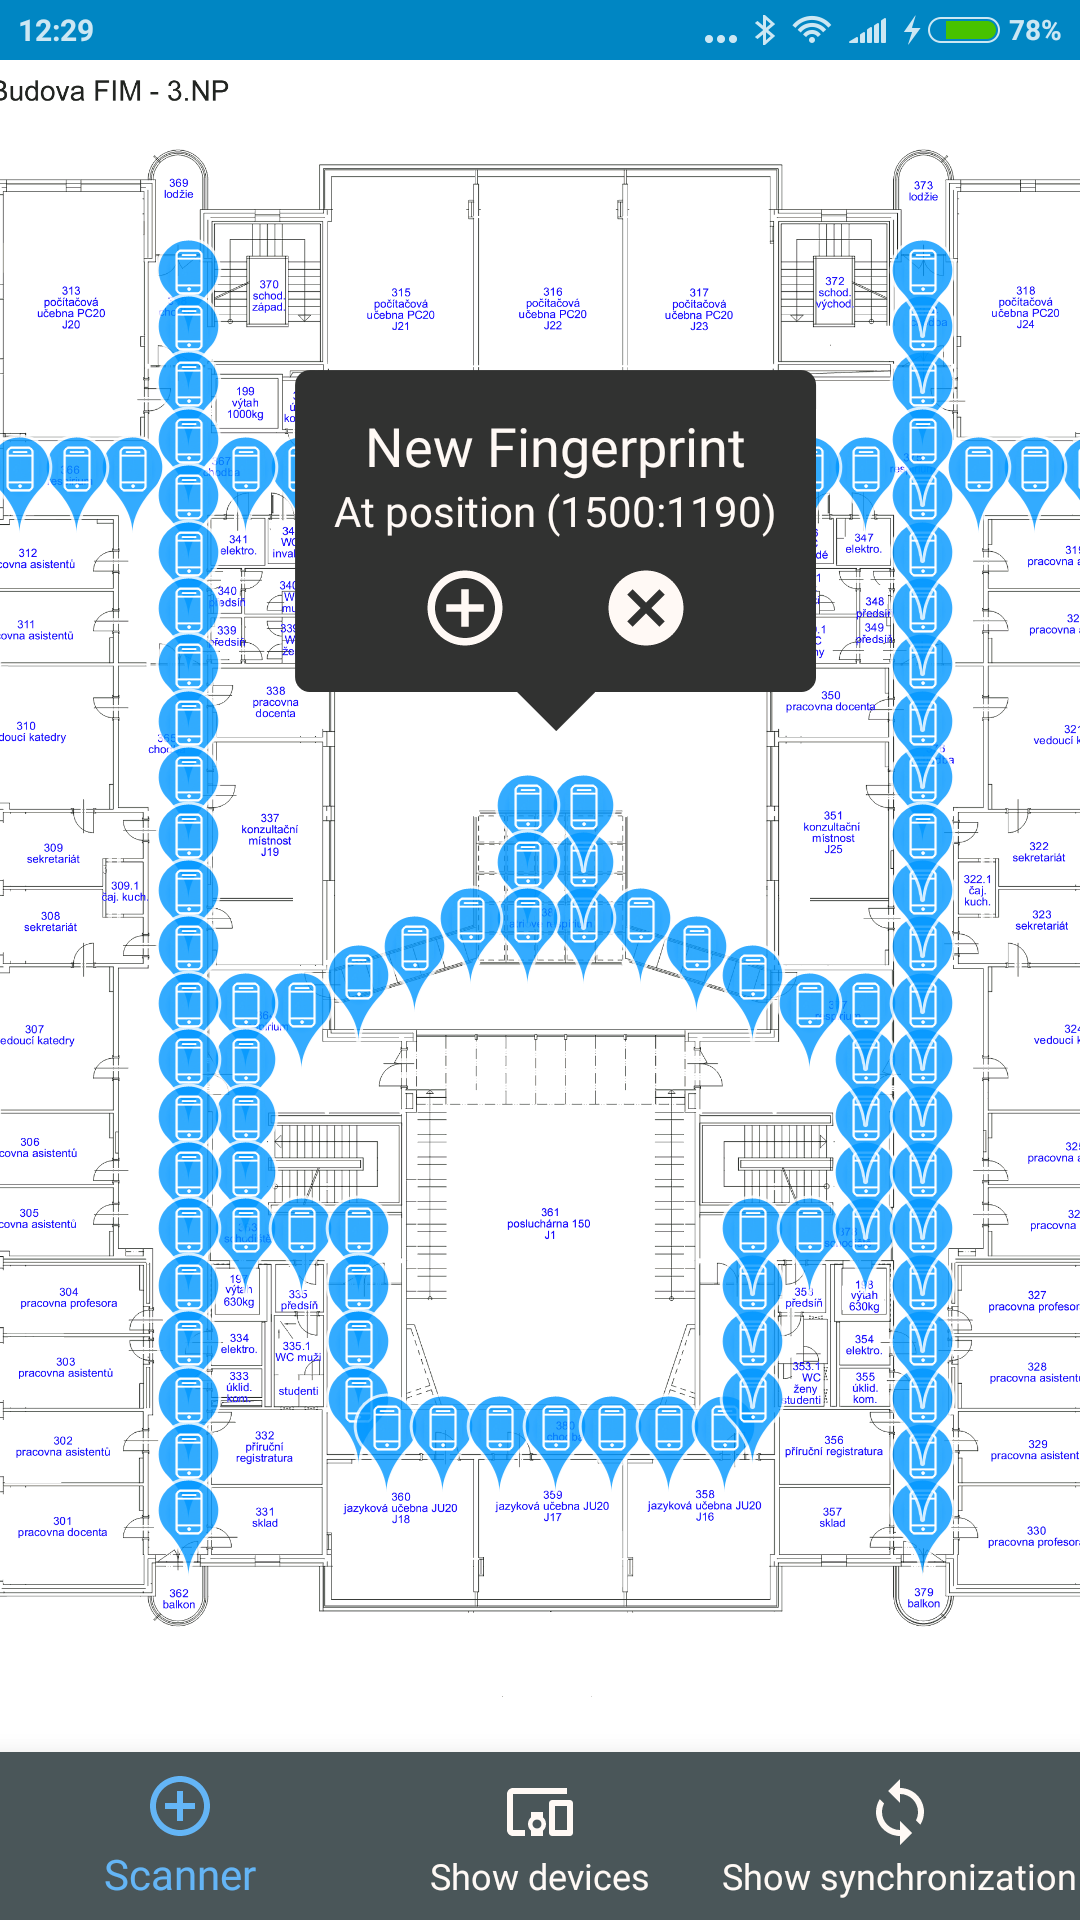
\includegraphics[width=0.30\textwidth]{img/map_markers}
		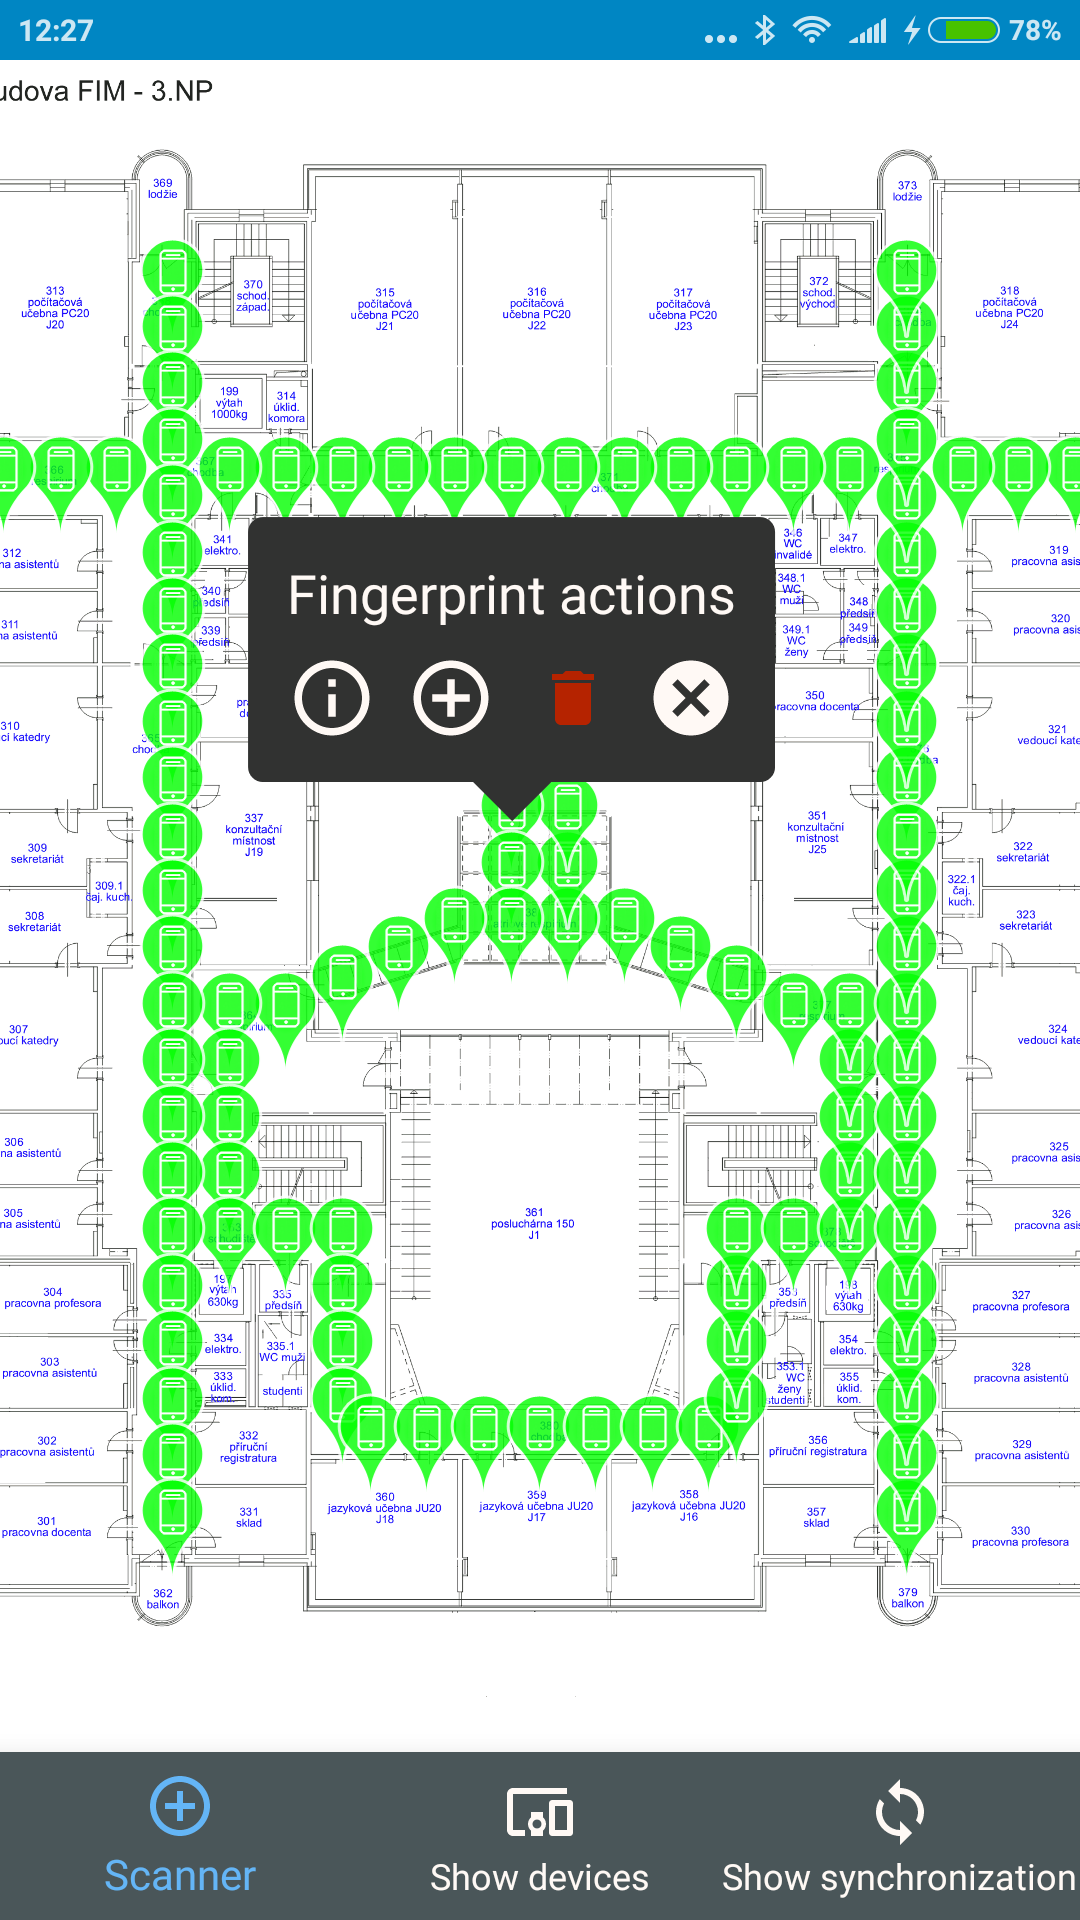
\includegraphics[width=0.30\textwidth]{img/map_markers_own}
		\par\end{centering}
	\caption{Map screen with markers\label{fig:map_with_markers}}
	\label{fig04c05}
\end{figure}

\fref{fig04c05} shows two screens of the map with markers, which are split by two colors and images. Color combination signifies if the latest fingerprint is from current device (green) or from another one (blue). This is based on fingerprint origin device, which is always mobile, meaning if wear displays as green then fingerprint originated on current mobile phone. Images combination distinguishes between device type, mobile or wear in this case.

Each spot on the map can be clicked, including markers, to display overlay with fingerprint actions. There are two different displays for this overlay. First, when user clicks on existing marker there are options to display information about that specific spot, containing list of the fingerprints, enable user to create new fingerprint on that spot, delete last group or hide this overlay. Second, is displayed when clicked spot does not have previously created fingerprints. This overlay displays only option to add new fingerprint or hide this window. Both of these options are displayed in \fref{fig04c05}.

Adding new fingerprints will create all necessary data for a scan and runs it via already mentioned JobScheduler. This scan has always priority, meaning if there is a non-priority scan running it is canceled and this one is run instead. This is the case when Devices screen initiated a scan which did not finish just yet. When this scan is running all application screens (Activities) display scan information as shown in the \fref{fig05c05}, thus informing about scan status in all parts of the application.

\begin{figure}[H]
	\begin{centering}
		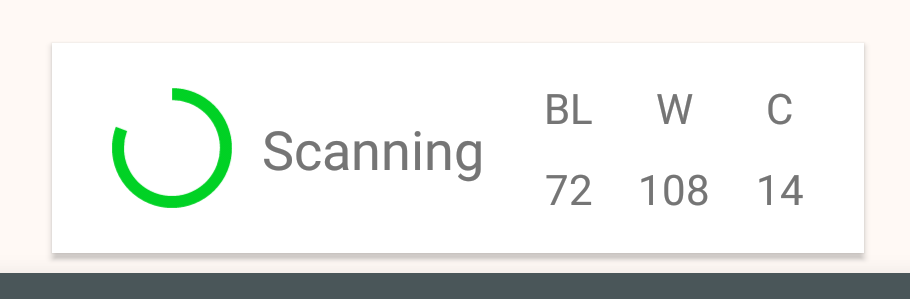
\includegraphics[width=0.6\textwidth]{img/scan_status}
		\par\end{centering}
	\caption{Scan status}
	\label{fig05c05}
\end{figure}

This information window overlays the screen just above the application menu. It informs user about scan status, progress and how many device records were saved until now. It displays information about BLE (B), WiFi (W) and Cellular (C) data collected but it does not show Sensor (S) information to save space.

Original map image has 3000 x 2200 pixels but with a low size around 230 kB so it could be displayed as a single image but for already mentioned reasons it is not. The image is cut into four zoom levels with first having 4 images and the final one with 144. Left side of \fref{fig06c05} shows maximum zoom on the mobile screen and right side displays information about fingerprint in a specific spot.

\begin{figure}[h!]
	\begin{centering}
		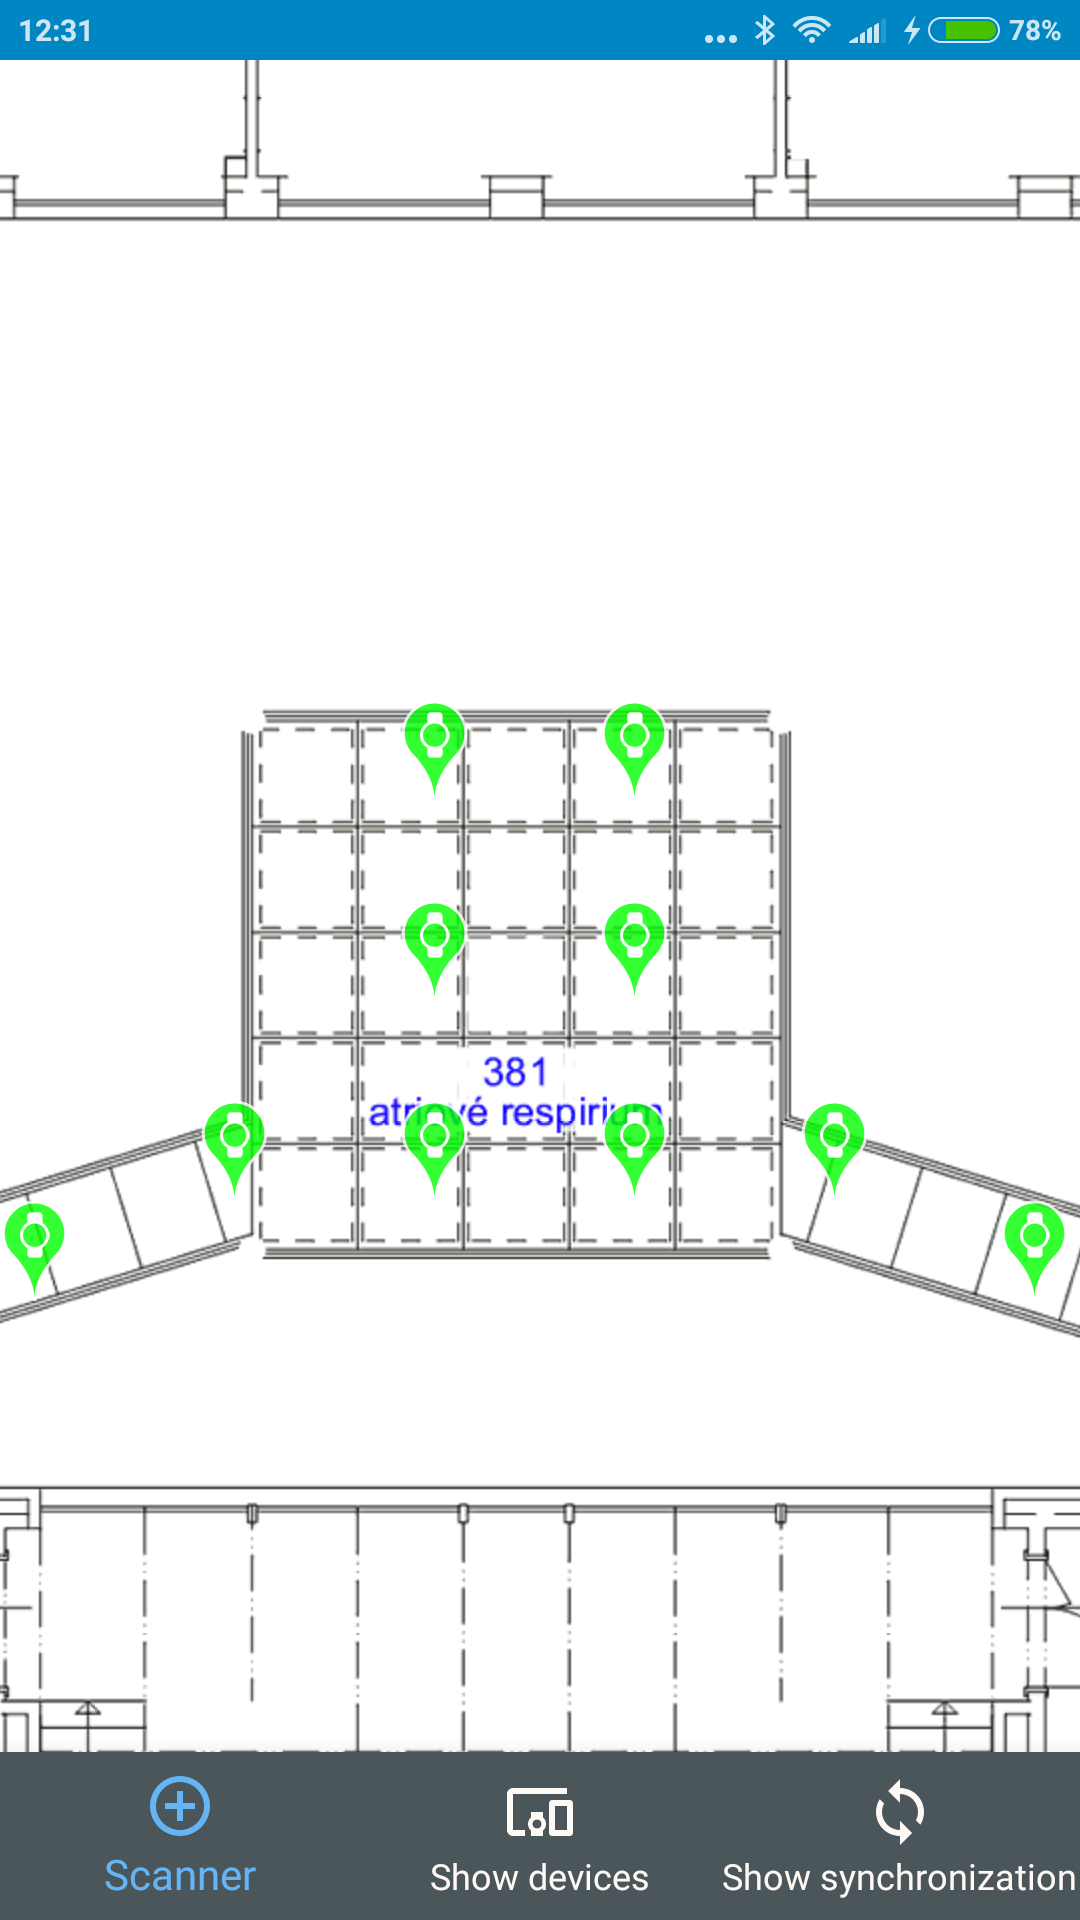
\includegraphics[width=0.30\textwidth]{img/map_zoom}
		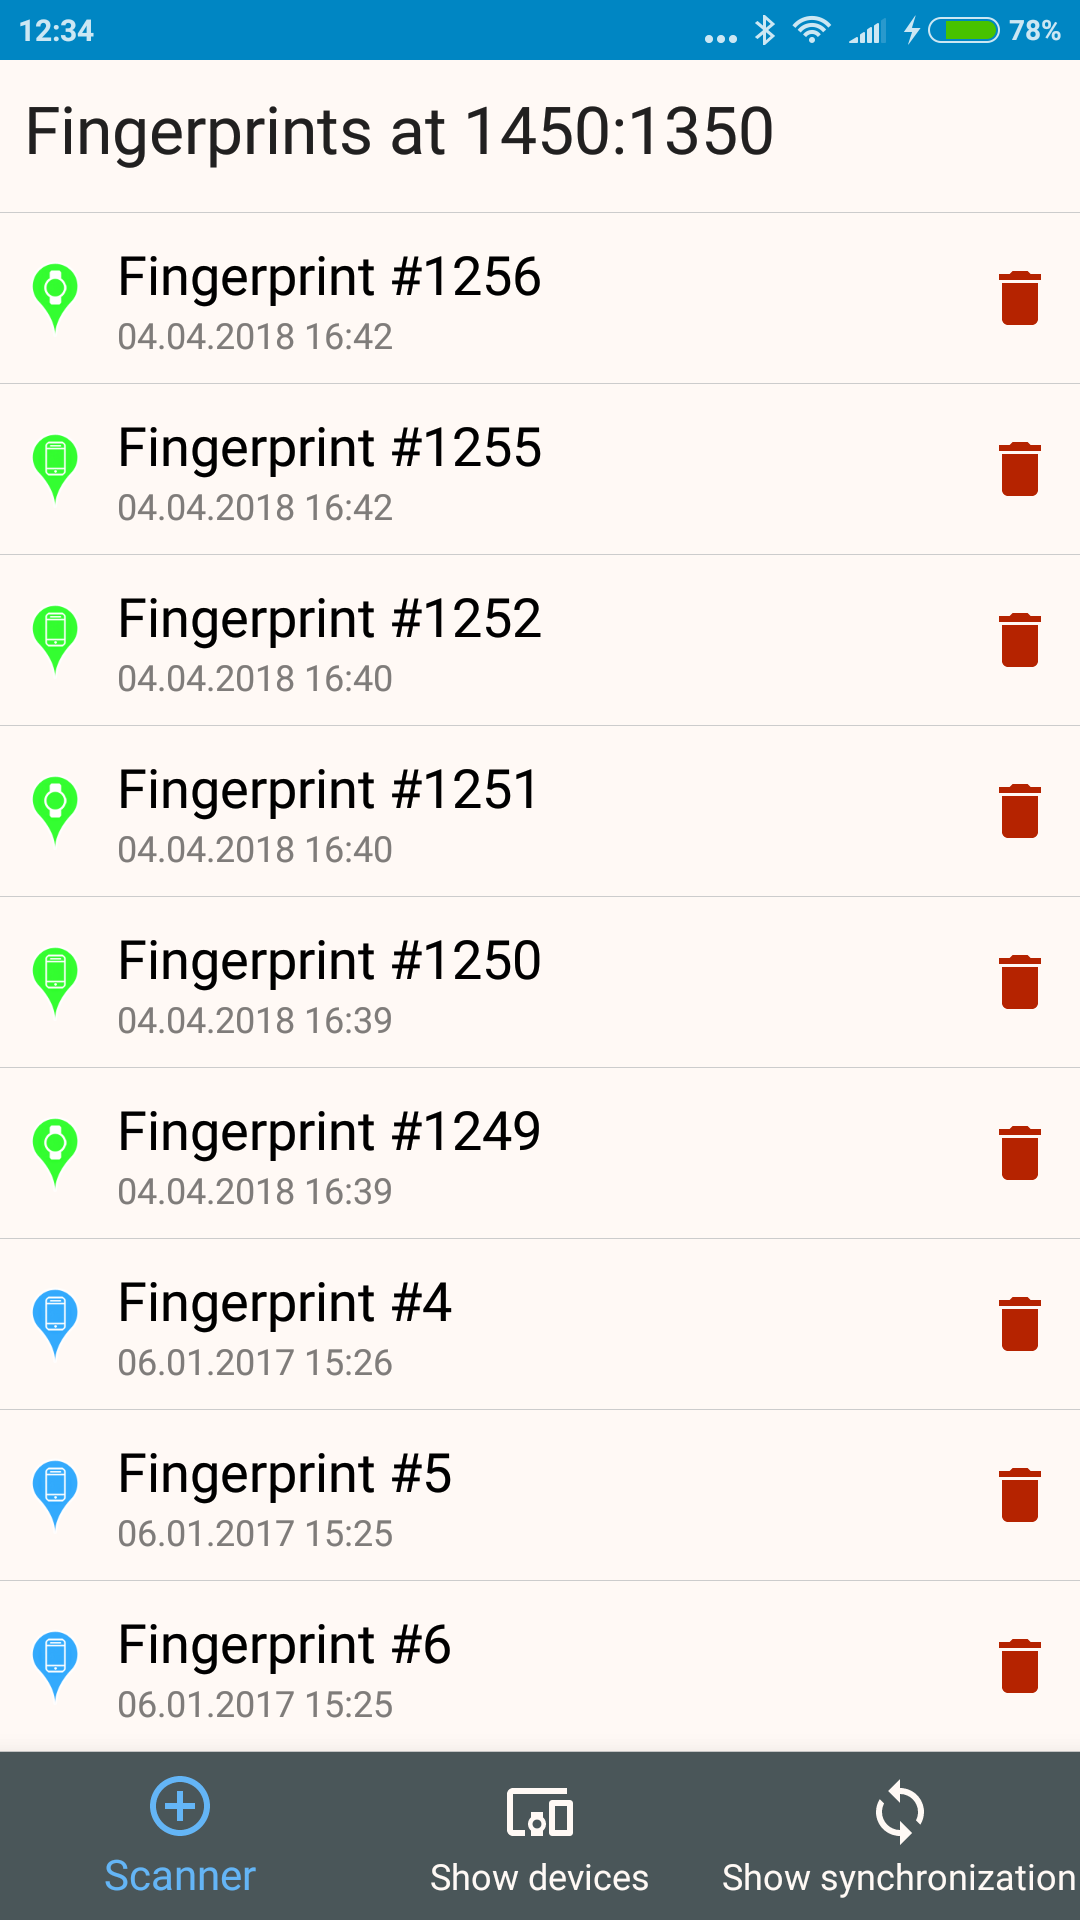
\includegraphics[width=0.30\textwidth]{img/map_list_fingerprints}
		\par\end{centering}
	\caption{Maximum map zoom (left), List of fingerprints (right)\label{fig:map_zoom_and_list}}
	\label{fig06c05}
\end{figure}

List of fingerprints for a specific spot displays information about origin device by icon, time it was created and enables to delete specific ones from the mobile. It is planned to extend this feature to display all important information about fingerprint, such as ids, device, counts of measurements and even RSSI averages. This would enable to assess fingerprint viability before uploading it on the server.

Important thing to note is deleting fingerprints will not be reported to the server, therefore deleting fingerprints is advised before uploading to the server. Deletion of already uploaded fingerprint on the phone will remove it only from that device and to delete it from the server is only enabled on the server itself. 

\subsubsection{Devices}\label{subsec:Devices}
It was supposed to be used for establishing connection between mobile and wearable device but this is done via Wear OS application and not necessarily required since Data Layer API and it also can send data between devices via WiFi. Even though it has no use it was kept to display surrounding devices and mainly BLE beacons.

\begin{figure}[h!]
	\begin{centering}
		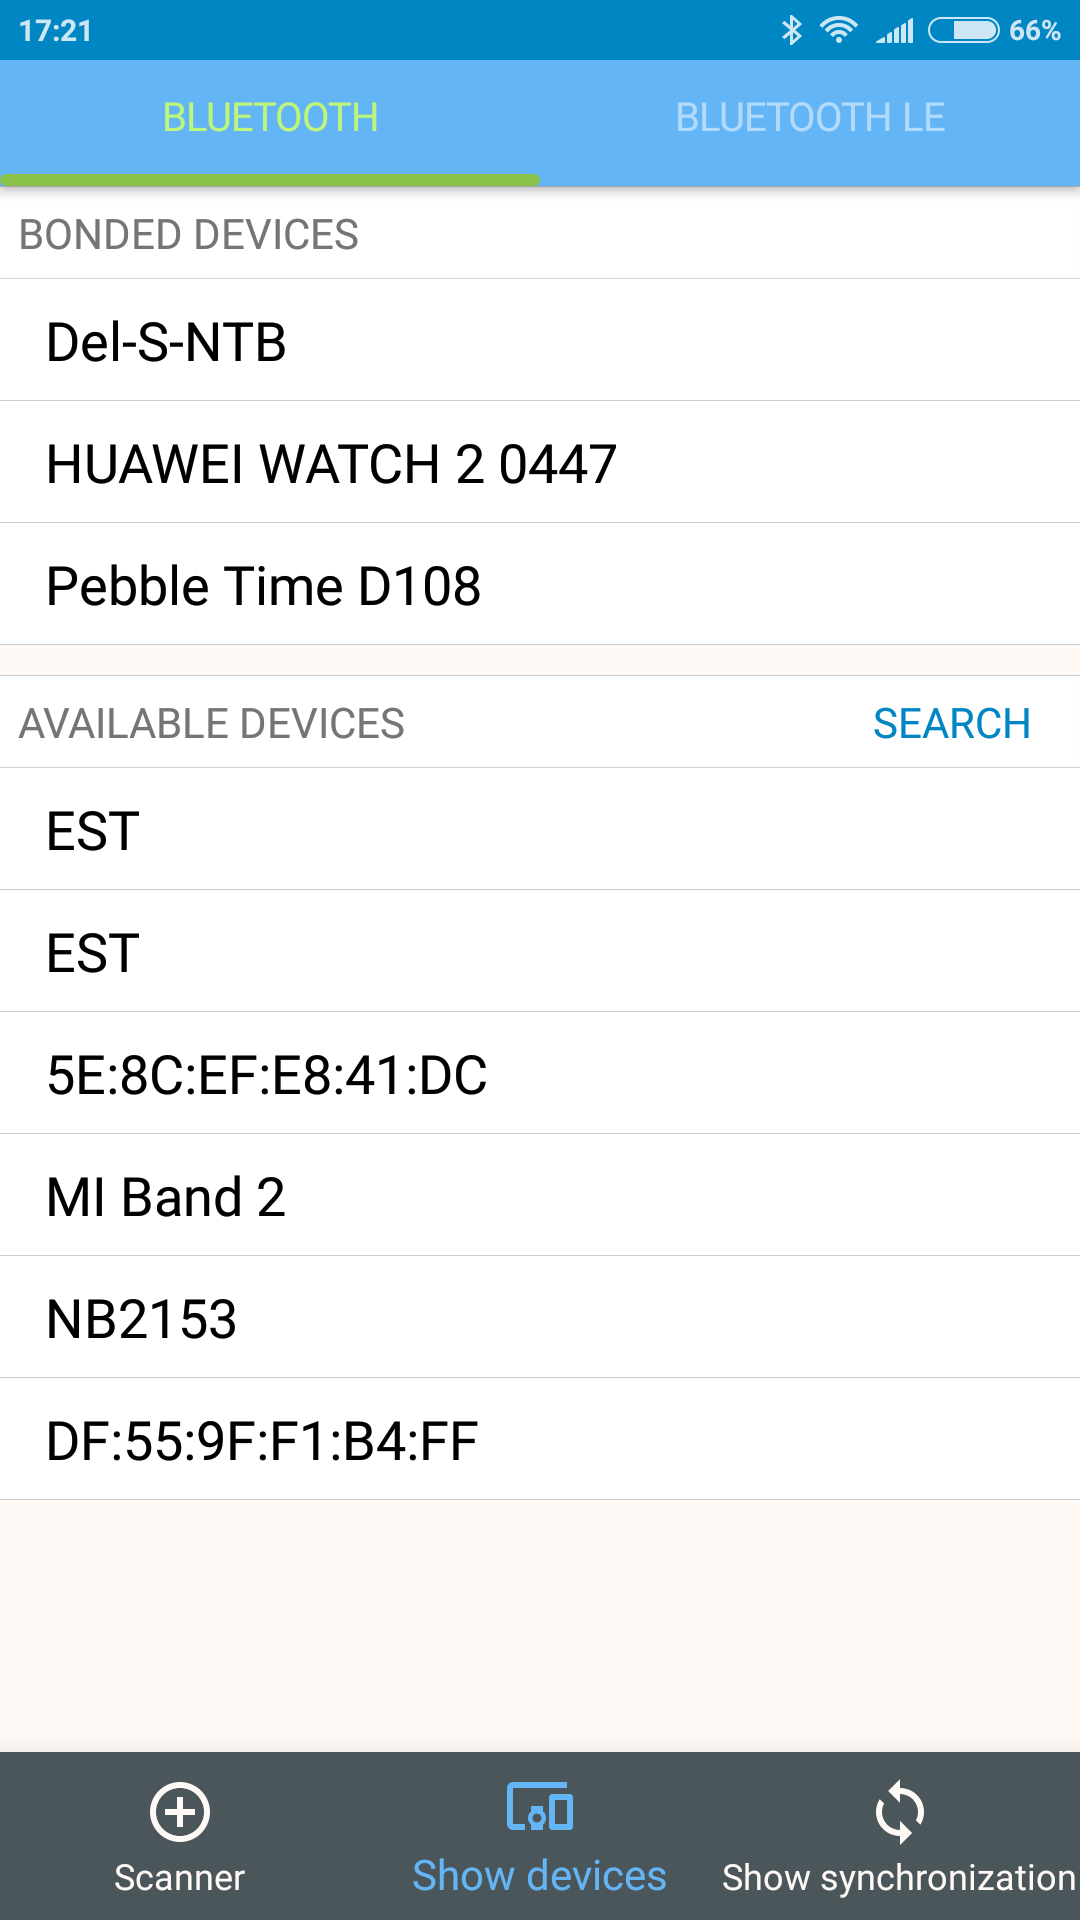
\includegraphics[width=0.30\textwidth]{img/devices_bl}
		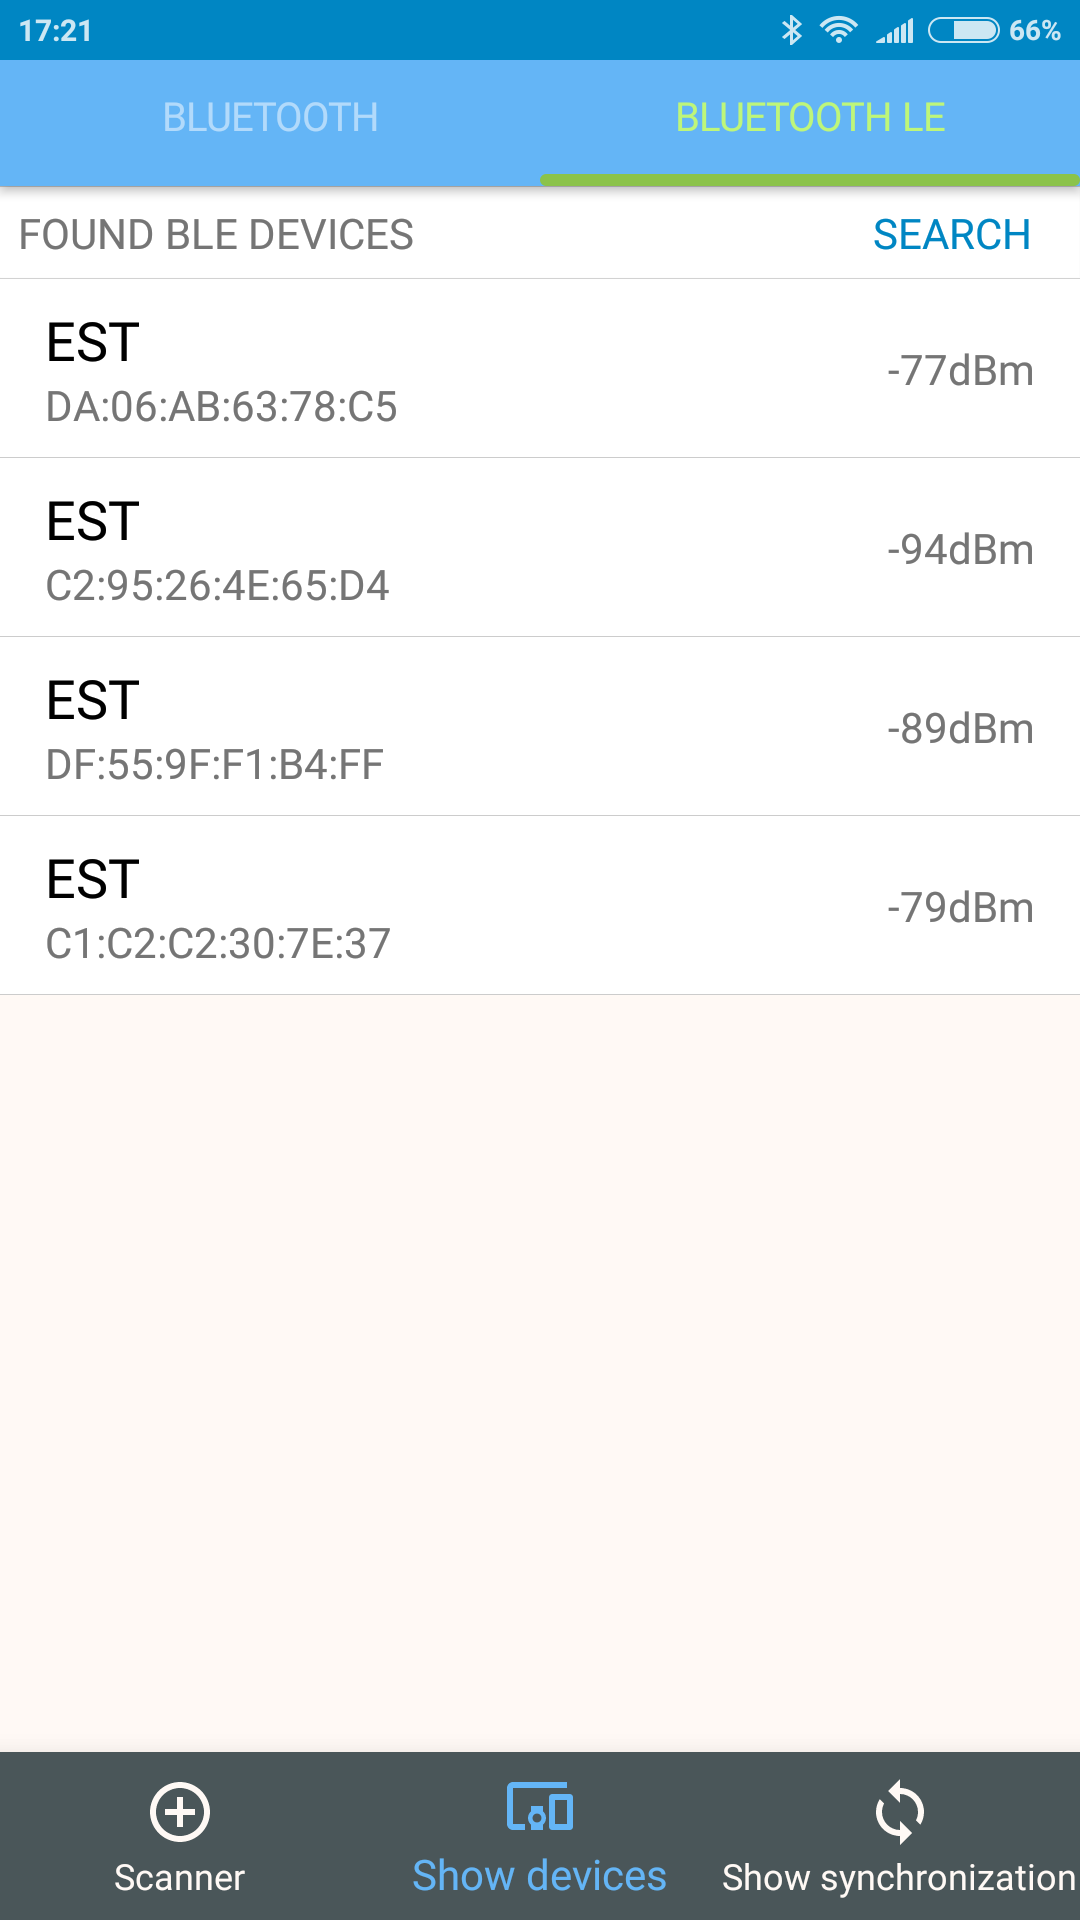
\includegraphics[width=0.30\textwidth]{img/devices_ble}
		\par\end{centering}
	\caption{Bluetooth devices (left), Beacons (right)\label{fig:bl_ble_list}}
	\label{fig07c05}
\end{figure}

Left screen of \fref{fig06c05} displays all the Bluetooth devices recorded during last scan, which is 15 seconds long. This scanning feature is not continuous and to display new devices it is needed to start the scan by pressing \enquote{Search} button, this will also clear the available devices list. There is no need to scan for bonded Bluetooth devices since Android keeps them in a separate list, which is good but it does not check if the device is in range or not, this it can display the device that is not available.

Right screen displays only devices broadcasting using Bluetooth Low Energy, those are mainly beacons but it can also be some TVs or wristbands. It displays basic information like name, mac address and last signal strength received. Same as Bluetooth list scanning is not continuous and is initiated by pressing \enquote{Search} button, length of such scan is set for 30 seconds in this case.

There is a possibility for both screens where device does not have a set name, in this case MAC address is displayed instead of missing name. To make this screen more viable it could display more information about devices, plus it could be extended to show WiFi access-points and Cellular towers in range.

\subsubsection{Synchronization}\label{subsec:Synchronization}
As the name suggests this screen is used to synchronize data between mobile and the server, it shows current fingerprint differences and enables data synchronization based on used input. It does not download or upload the data on its own since it is very data consuming, this it needs to be triggered by the user. Contrary to scanning information it does not display an overlay with the status, instead of that, after every successful upload or download is done it updates counts on the screen. It also shows an animation of top synchronization button and displays a message if it finished successful or failed.

\begin{figure}[H]
	\begin{centering}
		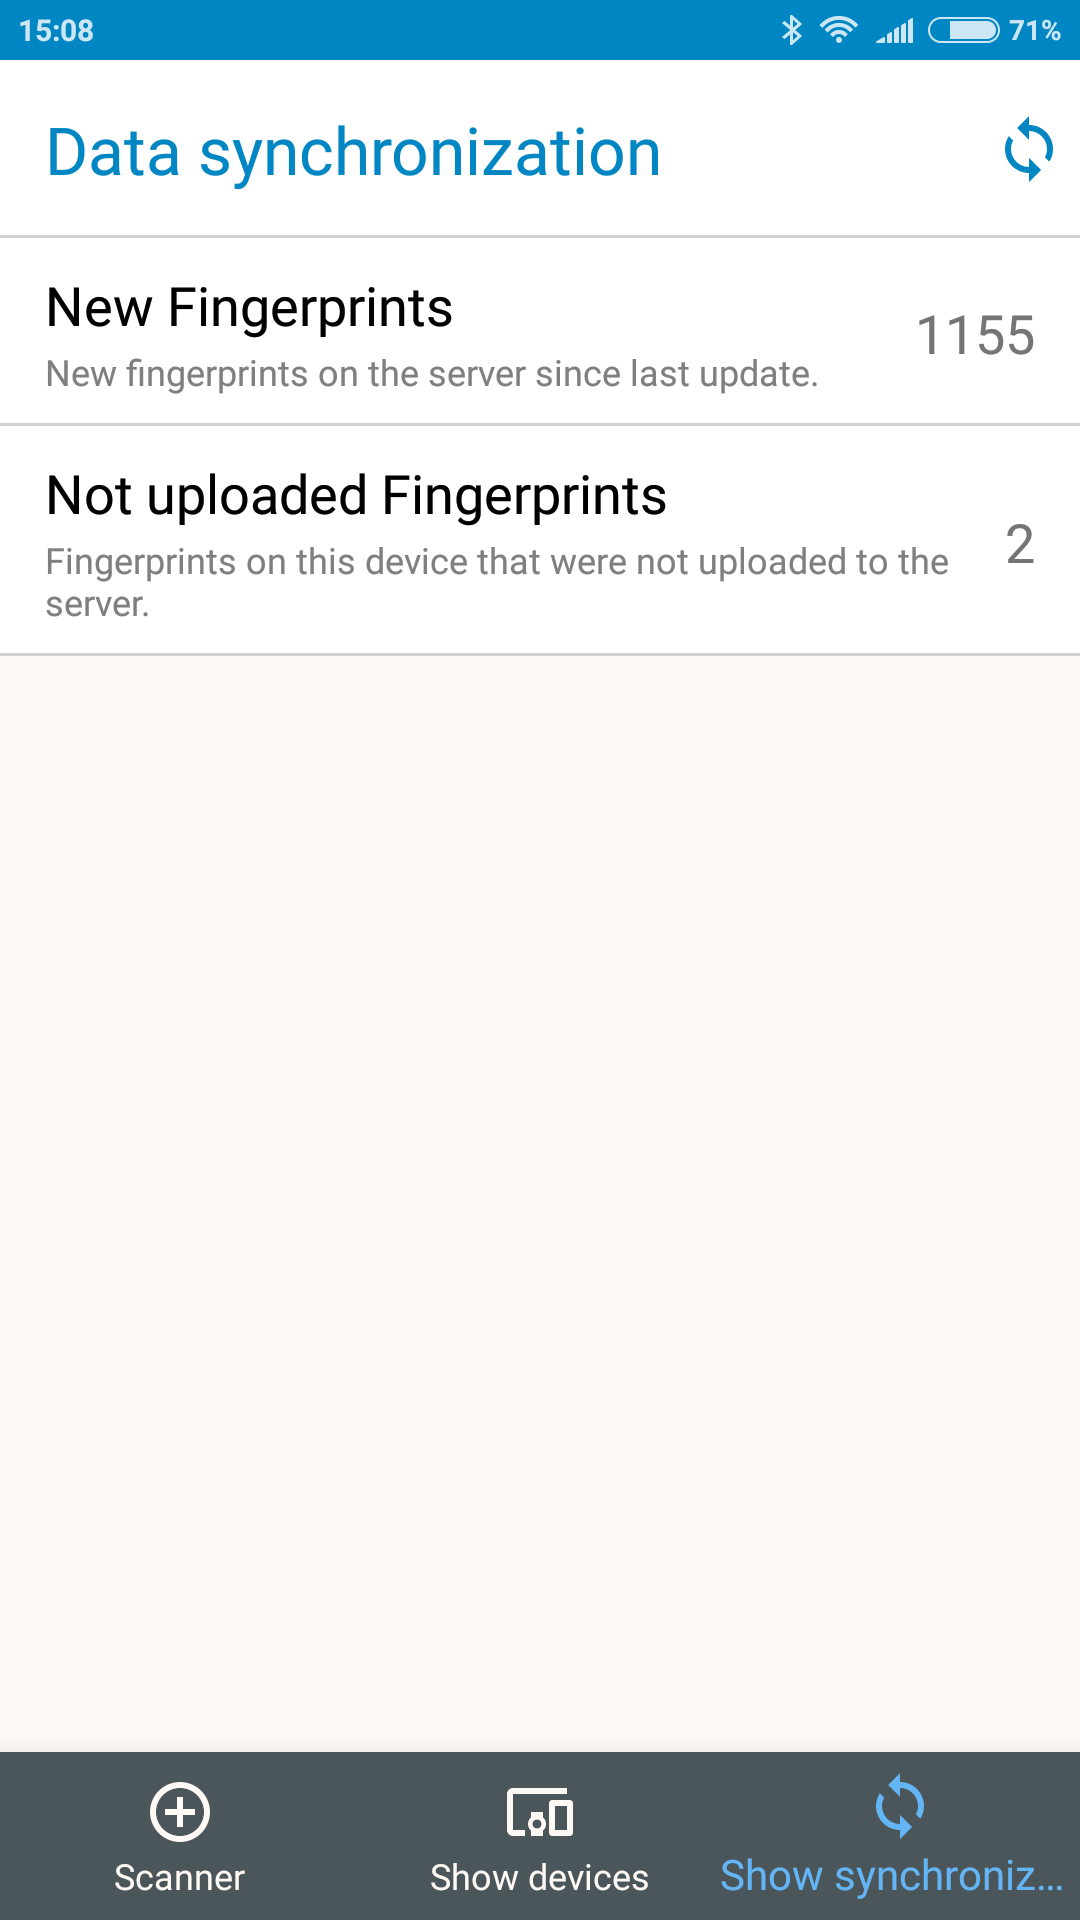
\includegraphics[width=0.3\textwidth]{img/synchronization}
		\par\end{centering}
	\caption{Synchronization screen}
	\label{fig08c05}
\end{figure}

It is planned to expand this screen for the use of application configuration to make it more flexible and able to be used in different environments than the current one. There are many changes considered which could influence the scanning results and application use.

\begin{itemize}
	\item Change scanning properties like maximum length, time periods for each scan or even make scanning periodic. There could also be different settings for wearable device.
	\item Enable to change server API address and download/upload limits. The API would have to implement same endpoints as current one in this case.
	\item Add map tiles uploading for different floors or buildings with the possibility to change between them and download fingerprints based on such location.
	\item User verifications for the application and API with the possibility to change them on this screen.
\end{itemize}

\subsubsection{Wear scanner}\label{subsec:WearableScanner}
Wearable application is meant to be as simple as possible. It has only a single screen since all the other settings are done on mobile application. This screen has two display states and holds device wake lock prevent screen dimming or turning off when there is a scan running. Only reason to keep this wake lock is to display scan information without the need to click on wear screen, this feature could be also implemented as optional with the possibility to change in the phone application settings (currently synchronization) screen. 

\begin{figure}[H]
	\begin{centering}
		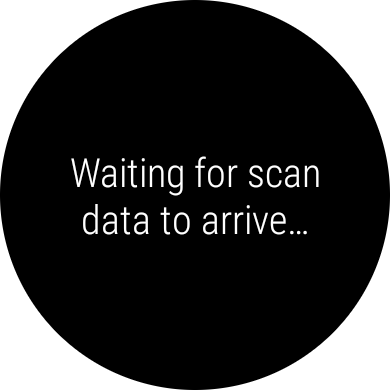
\includegraphics[width=0.3\textwidth]{img/wear_waiting_edited}
		\hspace{0.5cm}
		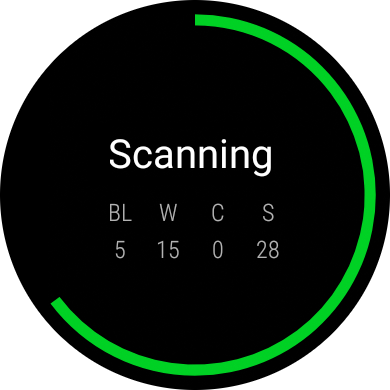
\includegraphics[width=0.3\textwidth]{img/wear_scanning_edited}
		\par\end{centering}
	\caption{Wear scanning screens}
	\label{fig09c05}
\end{figure}

First screen shows information message about receiving scan data from mobile, when no data is received for 10 seconds it is closed to reduce battery drain. Second screen displays scan status with a progress bar and count of scanned records. When a scan is completed the informations about it stays displayed for tree seconds, after this time the screen is reset to the first one and application is closed. Since the scan can be run with wear at a position where user is not able to check the data, it informs about scan start and end with a short device vibration.

\subsection{Interesting code examples}\label{subsec:Interesting code examples}
This application is collection of complex code and functions and some interesting parts were selected to describe in more detail.

\subsubsection{Sending Fingerprint to Wear}\label{subsubsec:SendingFingerprintToWear}
Core functionality of communication between both devices. This code can be found in a WearDataSender class of mobile application and it sends Fingerprint data to the wear using Data Layer API right after wear application is started.

\begin{lstlisting}[caption=Sending Fingerprint to Wear]
if(mFingerprint != null) {
	mFingerprint.setDeviceEntry(null);
	
	PutDataMapRequest dataMapRequest = PutDataMapRequest.create(DataLayerListenerService.SCAN_PATH);
	DataMap dataMap = dataMapRequest.getDataMap();
	ParcelableUtils.putParcelable(dataMap, DataLayerListenerService.SCAN_DATA, mFingerprint);
	
	PutDataRequest request = dataMapRequest.asPutDataRequest();
	request.setUrgent();
	Wearable.getDataClient(mContext).putDataItem(request);
	
	mFingerprint = null;
}
\end{lstlisting}

Since this class handles starting wear application and also sending the data it has Fingerprints saved as a global variable and to be send it must not be empty. Only one change is done to the fingerprint before it is send, which is removing of origin device information to be filled in the wear. When fingerprint is prepared it must be converted into Parcelable DataMap which is an object that is saved into the Data Layer. This data is identified by a String key so application can save multiple objects into this map. Next part of code creates a request using this data and sets its mode to urgent to ensure fast delivery to all devices that listen to this information. Request is completed at this point and can be send via DataClient which can be loaded from the class Wearable wit final line of code clearing the variable containing fingerprint to prevent its sending multiple times.

Data Layer identifies all the data by a specific Uri and when the data is changed it sends an information to all devices, meaning each fingerprint must be different for sending notification about data change to the devices. Luckily every fingerprint has its own specific id and scan id which is always different so this feature does not pose any problem to the data sending.

\subsubsection{Parsing beacon information}\label{subsubsec:ParsingBeaconInformation}
None of the scanner parts uses default classes to contain scanned information. With each class custom data must be parsed from default ones during the scanning and following code, taken from FingerprintScanner class, shows how to parse beacon data.

\begin{lstlisting}[caption=Parsing beacon information]
String bssid = beacon.getBluetoothAddress();

long scanTime = currentMillis - mStartTime;
if(scanTime == currentMillis) {
	scanTime = 0;
}
long scanDifference = calculateBeaconScanDifference(scanTime, bssid);

BeaconEntry newBeacon = new BeaconEntry();
newBeacon.setBssid(bssid);
newBeacon.setDistance((float) beacon.getDistance());
newBeacon.setRssi(beacon.getRssi());
newBeacon.setTimestamp(currentMillis);
newBeacon.setScanTime(scanTime);
newBeacon.setScanDifference(scanDifference);

return newBeacon;
\end{lstlisting}

First loaded information is device mac address because it is used to calculate time differences between the last time recorded and current time which is done in following part. After all time values are calculated BeaconEntry can be created containing all required data and immediately returned.

Setting scanTime to 0 works as a protection against having it the same as currentMillis because start time of the scan might not have been set just yet. This is needed mainly for WiFi scanning because these parsing classes have to be set just before running scanner code which leaves few milliseconds where data can be started before scan is actually stared considering WiFi scan cannot be controlled. It could be also solved by not recording this data but since it is only a milliseconds space it was decided that environment will not change enough to make the data irrelevant and so they are recorded too.

\subsubsection{Map configuration}\label{subsubsec:MapConfiguration}
Map is the main part of the application and handles multiple functions and mode thus required a lot of the settings to work properly. It also has many functions which can be configured or disabled based on the implementation required. This map and the code is implemented in MapFragment class.

\begin{lstlisting}[caption=Map configuration]
mMap.setSize(MAP_WIDTH, MAP_HEIGHT);
mMap.addDetailLevel(1.000f, "tiles/j3np/1000/j3np-%d_%d.png");
mMap.addDetailLevel(0.500f, "tiles/j3np/500/j3np-%d_%d.png");
mMap.addDetailLevel(0.250f, "tiles/j3np/250/j3np-%d_%d.png");
mMap.addDetailLevel(0.125f, "tiles/j3np/125/j3np-%d_%d.png");

mMap.setScaleLimits(0, 2); 
mMap.setScale(0.50F);

... Setup markers and hotspots ...

frameTo(MAP_WIDTH / 2, MAP_HEIGHT / 2);

mMap.setShouldRenderWhilePanning(true);
mMap.setShouldLoopScale(false);
\end{lstlisting}

First part contains setting map size which is 3000x3000 pixels and configure zoom levels with their specific tile images based on given path, setting zoom levels one by one makes it highly modifiable with the possibility to have different designs for each zoom level. Next part sets zoom values, such as allowed zoom levels and initial zoom of the map. Next part is setting up markers and hotspots which will be described later. Calling function frameTo centers the map with a delay because if is done directly it will not work. Final part of this code enables loading when map is panning and disables returning to maximum zoom after double clicking while being zoomed in, be on zoom level 2 in this case.

\begin{lstlisting}[caption=Setup markers and hotspots]
mMap.setMarkerTapListener(mMarkerTapListener);
mMap.defineBounds(0, 0, MAP_WIDTH, MAP_HEIGHT);
mMap.setMarkerAnchorPoints(-0.5f, -0.5f);

HotSpot hotSpot = new HotSpot();
hotSpot.set(0, 0, MAP_WIDTH, MAP_HEIGHT);
mMap.addHotSpot(hotSpot);
mMap.setHotSpotTapListener(mHotspotTapListener);
\end{lstlisting}

First part of the code sets variables for map markers, such as displaying control window after clicking, define bounds and anchor point for marker centering in horizontally and vertically. Defining bounds to the markers is very important information because it enables to calculate real pixel location from map absolute one since location on the map changes based on how much the map is zoomed but for scanning the real fingerprint location is needed.  This code does not actually display any markers on the map that is done later in the code.

Second part works similarly to previous one but it does not set the click function only to markers but creates an invisible overlay over the whole map, thus effectively enabling to click on any part of the map to display control window for fingerprints.